%%%%%%%%%%%%%%%%%%%%%%%%%%%%%%%%%%%%%%%%%%%%%%%%%%%%%%%%%%%%%%%%%%%%%%%%
\chapter{Introduction}
\label{cht:intro}

The purpose of this document is to discuss observation models
used in nonlinear mixed effects (NLME) models for continuous data 
and supported in PharmML, \cite{Pharmml_06}. It starts with a 
general classification of observation models and discusses aspects of the 
variability structure of residual error models.
A short overview of the most common models follows which are then 
described in detail in chapter \ref{sec:typicalResModel}. Chapter \ref{ch:otherModels} 
discusses then a number of non-standard models, among others from the 
\cite{Keizer:2013aa}.


\section{Classification of observation models} % \textcolor{red}{changes}
\label{sec:modelClassific}

The observation models can be divided into three groups:
\begin{itemize}
\item 
\textbf{Structured} models (\textbf{S-type})
\begin{itemize}
\item 
\textbf{General model} -- residual error, $\epsilon_{ij}$, with a symmetric distribution with mean 0
\begin{itemize}
 \item
for \textbf{transform-both-sides} data
\begin{eqnarray}
 \underbrace{ u(y_{ij})}_{\text{\parbox{2cm}{\centering Transformed \\[-4pt] experimental \\[-4pt]  data}}} =
 \underbrace{ u\big(f(x_{ij}, \psi_{i})\big)}_{\text{\parbox{2.5cm}{\centering Transformed \\[-4pt]  model \\[-4pt]  prediction}}} +
 \underbrace{ g(x_{ij}, \psi_{i}, \xi_i) \; \epsilon_{ij}}_{\text{\parbox{3cm}{\centering Residual \\[-4pt] error}}}
 \end{eqnarray}
\item
for \textbf{untransformed} data  -- special case of the previous with $h \equiv identity$ 
\begin{eqnarray}
 \underbrace{ y_{ij}}_{\text{\parbox{2cm}{\centering Experimental \\[-4pt]  data}}} =
 \underbrace{ f(x_{ij}, \psi_{i})}_{\text{\parbox{2.5cm}{\centering Model \\[-4pt]  prediction}}} +
 \underbrace{ g(x_{ij}, \psi_{i}, \xi_i) \; \epsilon_{ij}}_{\text{\parbox{3cm}{\centering Residual \\[-4pt] error}}}
 \nonumber
 \end{eqnarray}
\end{itemize}
\item
\textbf{Gaussian model} --  special case of eq. (1.1) with $\epsilon_{ij} \sim \mathcal{N}(0,1)$ --
$u(y_{ij})$ is normally distributed with mean $u(f(x_{ij}, \psi_{i}))$ and the 
standard deviation $g(x_{ij}, \psi_{i}, \xi_i)$. 

\end{itemize}
\item 
\textbf{Distribution} based models (\textbf{D-type})
\begin{align}
	& u(y_{ij})  \sim DistributionName(parameter1, parameter2, ...)
\end{align}
\item
\textbf{Equation} based models  (\textbf{E-type})
\begin{eqnarray}
 \underbrace{ u(y_{ij})}_{\text{\parbox{2cm}{\centering Transformed \\[-4pt] experimental \\[-4pt]  data}}} =
 \underbrace{ U\big(f(x_{ij}, \psi_{i}),\xi_i, \epsilon_{1,ij}, \epsilon_{2,ij}, \dots\big)}_{\text{\parbox{3.5cm}{\centering Transformed \\[-4pt]  model prediction \\[-4pt]  including residual errors}}}
 \end{eqnarray}
\end{itemize}
Symbol description:
\begin{itemize}
\item	
$1\le i \le N$
\item
$1\le j \le n_i$
\item
$y_{ij}$ -- $j^{th}$ observation for subject $i$
\item
$f$ -- structural model prediction
\item
$x_{ij}$ -- regression variables, e.g. time or concentration
\item
$\psi_{i}$ -- individual parameters
\item
$\epsilon_{ij}$ -- normalised residual error
\item
$g$ -- standard deviation of the residual error
\item
$\xi_i$ -- parameters of the residual model.
\end{itemize}
%Type (1) is a special case of type (2) with $u \equiv Id$, i.e. the identity transformation. 
%Then for models of type (1) and (2) with $\epsilon_{ij}$ being normal distributed with 
%mean 0 and variance 1, 

%\subsection{Note of BTS - FINISH}
%Models for the standard deviation $g(x_{ij}, \psi_{i}, \xi_i)$ discuss in previous 
%section apply also in the case of \textbf{transform-both-sides} approach.
%\paragraph{Note}
%Models listed below are the most popular ones in use but the present PharmML 
%structure allows for implementation of virtually any user-defined transformation.

%\subsection{Classification and interoperability}
%\label{sec:interopGoals}
%


\section{Variability structure}
\label{sec:variabStructure}
In most cases the variability structure is reduced to one level, that of the 
observation, and its magnitude is equal among the entire population. 
However, in general, the magnitude of the residual error can vary between 
subjects or occasions. Essay errors are another variability source, the  
so called inter-replicates variability.

\subsection{Inter-individual/occasion variability (IIV/IOV)}
\label{subsec:IIVonResidualError}
In analogy to the nested hierarchical structure for the variability of the 
individual parameters, see \cite{Pharmml_06}, the variability of residual 
error parameters inherits the same structure. This way one can capture 
the inter-individual and/or inter-occasion variability of the residual error parameters.
The IIV on the residual error parameters, i.e. the varying magnitude of 
residual error between subjects, corresponds to the so 
called 'ETA-on-EPS' approach, see Figure \ref{fig:IOV0_residualError}.

\begin{figure}[htb!]
\centering
  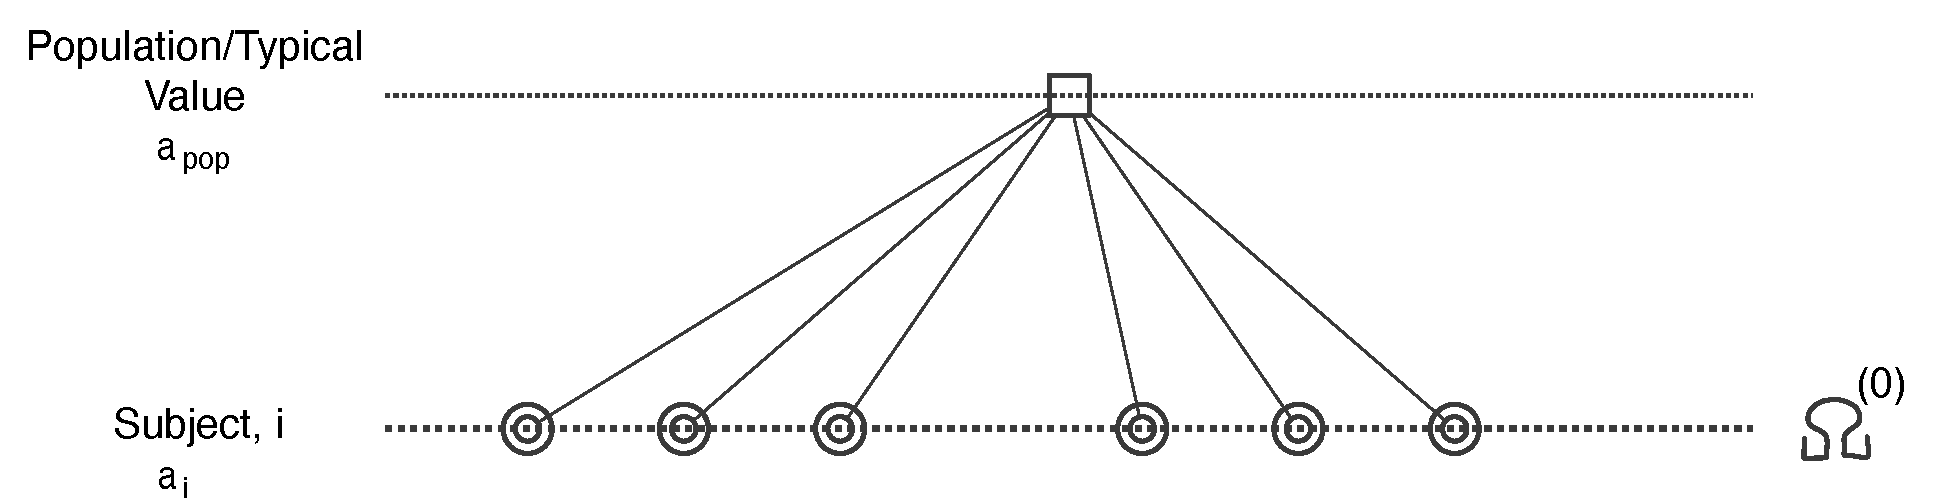
\includegraphics[width=140mm]{pics/IOV0_residualError.pdf}
 \caption{Inter-individual variability of the residual error parameter, $a$, visualised 
 as basic nested hierarchy.}
 \label{fig:IOV0_residualError}
\end{figure}

For example, if additive residual error model and log-normal distribution 
for $a$ is assumed, then the parameter model reads
\begin{eqnarray}
	&& \log(a_i) \sim \mathcal{N}(\log(a_{pop}) , \omega_a^2) \nonumber
\end{eqnarray}
and the observation model reads
\begin{eqnarray}
	&& y_{ij} \sim \mathcal{N}(f_{ij},a_i^2): \quad y_{ij} = f_{ij} + a_i \epsilon_{ij}, \quad \epsilon_{ij} \sim \mathcal{N}(0,1)	\nonumber
\end{eqnarray}
See also chapter \ref{ch:otherModels} for IIV and IOV examples with NMTRAN and MLXTRAN code.

\subsection{Inter-replicate variability (IRV)}
This variability type is analog to the inter-occasion variability for parameters,
see for example \cite{LavielleBook:2014}, and has been first considered and described in the 
literature by \cite{Karlsson:1995rm}. The replicate level in this residual error 
is described by an additional random effect and reads  
\begin{eqnarray}
	&& y_{ijk} = f_{ij} + \epsilon_{ij} + \epsilon_{ijk}, \text{ with } \epsilon_{ij} \sim \mathcal{N}(0,\Sigma^{(0)}), \epsilon_{ijk} \sim \mathcal{N}(0,\Sigma^{(1)}) 	\nonumber
\end{eqnarray}
with the $k$ index for the replicates and can therefore be visualised graphically 
in a very clear nested hierarchical structure, Figure \ref{fig:IRV_residualError}.
\begin{figure}[htb!]
\centering
  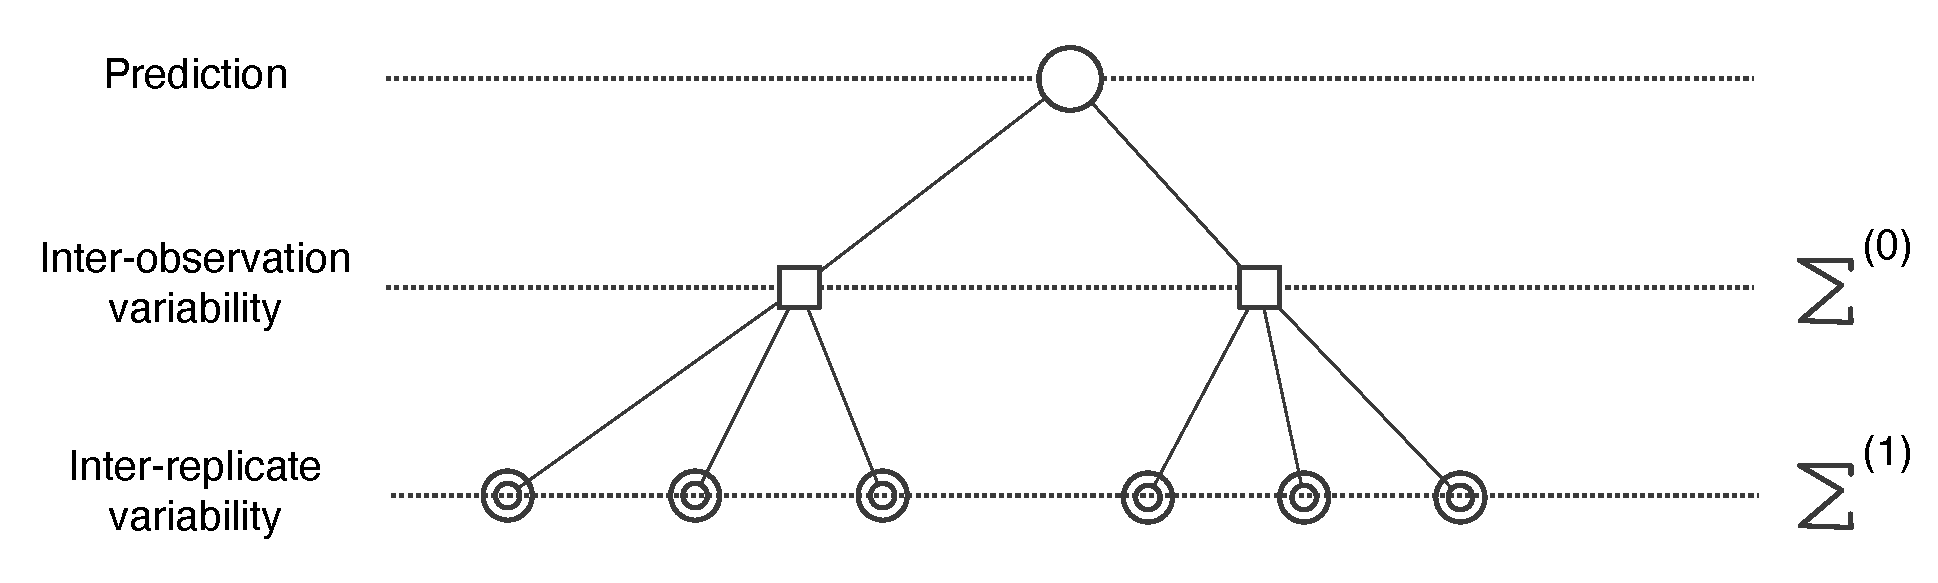
\includegraphics[width=140mm]{pics/IRV_residualError}
 \caption{Inter-replicate variability in the residual error, visualised 
 as nested hierarchy.}
 \label{fig:IRV_residualError}
\end{figure}
Each level can be fully described by a covariance matrix, $\Sigma$.

\smallskip
See also chapter \ref{ch:otherModels} for IRV examples with NMTRAN and MLXTRAN code.

\section{Selected observation model types}
In the following we list a selection of commonly used observation/residual error models, 
based mainly on \cite{NONMEM:2006aa} and \cite{LavielleBook:2014}, and described 
in detail in the next chapters:
\begin{enumerate}
\item
Constant/additive:
\begin{center} $y_{ij} = f_{ij} + a \; \epsilon_{ij}; \quad \epsilon_{ij} \sim N(0,1)$ \end{center}
\begin{center} OR $\quad y_{ij} = f_{ij} + \epsilon_{ij}; \quad \epsilon_{ij} \sim N(0,\sigma^2)$ \end{center}
\item
Constant/additive for log-transformed data, aka \emph{exponential}:
\begin{center} $\log(y_{ij}) = \log(f_{ij}) + a \epsilon_{ij}; \quad \epsilon_{ij} \sim N(0,1) \Longleftrightarrow  y_{ij} = f_{ij} \exp(a\,\epsilon_{ij})$ \end{center}
\item
Constant/additive for logit-transformed data:
\begin{center} $\displaystyle\log\Big(\frac{y_{ij}}{1-y_{ij}}\Big) = \log\Big(\frac{f_{ij}}{1-f_{ij}}\Big) + g\epsilon_{ij} \Longleftrightarrow y_{ij} = \frac{f_{ij} \exp(g\,\epsilon_{ij})}{1+f_{ij}\big(\exp(g\,\epsilon_{ij}) - 1\big)}$ \end{center}
\item
Constant/additive for extended-logit-transformed data: 
\begin{center} $\displaystyle\log\Big(\frac{y_{ij} - A}{B-y_{ij}}\Big) = \log\Big(\frac{f_{ij}-A}{B-f_{ij}}\Big) + g\,\epsilon_{ij} 
 \Longleftrightarrow y_{ij} = A + (B-A) \frac{f_{ij}-A}{f_{ij} - A + (B-f_{ij})\exp(-g\,\epsilon_{ij})} $ \end{center}
\item
Constant/additive for Box-Cox transformed data: 
\begin{center} $
\left\{ \begin{array}{lcl}  \big(y_{ij}^\lambda - 1\big)/\lambda = \big(f_{ij}^\lambda - 1\big)/\lambda + g\,\epsilon_{ij} & \mbox{for} & \lambda  \neq 0  \\
\log(y_{ij})  = \log(f_{ij}) + g\,\epsilon_{ij}  & \mbox{for} & \lambda = 0
\end{array}\right.
\Longleftrightarrow \left\{ \begin{array}{lcl}  y_{ij} = \big(f_{ij}^\lambda + \lambda g\, \epsilon_{ij} \big)^{1/ \lambda}& \mbox{for} & \lambda \neq 0  \\
y_{ij} = f_{ij} \exp(g\,\epsilon_{ij})  & \mbox{for} & \lambda  = 0
\end{array}\right.$
\end{center}
\item
Proportional or constant coefficient of variation (CCV):
\begin{center}  $y_{ij} =  f_{ij} + bf_{ij} \; \epsilon_{ij}; \quad \epsilon_{ij} \sim N(0,1)$ \end{center}
\begin{center} OR $\quad y_{ij} =  f_{ij}(1+\epsilon_{ij}); \quad \epsilon_{ij} \sim N(0,\sigma^2)$ \end{center}
\item
Combined proportional 1:
\begin{center}  $y_{ij} =  f_{ij} + (a + bf_{ij}) \; \epsilon_{ij}; \quad \epsilon_{ij} \sim N(0,1)$ \end{center}
\item
Combined proportional 2:
\begin{center}  $y_{ij} =  f_{ij} + \sqrt{a^2 + b^2f_{ij}^2} \; \epsilon_{ij}; \quad \epsilon_{ij} \sim N(0,1)$ \end{center}
\begin{center} OR $\quad y_{ij} =  f_{ij} +  a\, \epsilon_{1,ij} + b f_{ij}\, \epsilon_{2,ij}; \quad \epsilon_{1,ij} \sim N(0,1); \quad \epsilon_{2,ij} \sim N(0,1) $ \end{center}
\begin{center} OR $\quad y_{ij} =  f_{ij} (1 + \epsilon_{1,ij}) + \epsilon_{2,ij}; \quad \epsilon_{1,ij} \sim N(0,\sigma_1^2); \quad \epsilon_{2,ij} \sim N(0,\sigma_2^2)$ \end{center}
\item
Power error model: 
\begin{center}  $y_{ij} = f_{ij} + b\,f_{ij}^c \; \epsilon_{ij}; \quad \epsilon_{ij} \sim N(0,1)$ \end{center}
\begin{center}  OR $y_{ij} = f_{ij} + f_{ij}^c \; \epsilon_{ij}; \quad \epsilon_{ij} \sim N(0,\sigma^2)$\end{center}
\item
Combined power error model 1:
\begin{center}  $y_{ij} =  f_{ij} + (a + b f_{ij}^c) \; \epsilon_{ij}; \quad \epsilon_{ij} \sim N(0,1)$ \end{center}
\item
Combined power error model 2:
\begin{center}  $y_{ij} = f_{ij} + a\epsilon_{1,ij} + b f_{ij}^c \epsilon_{2,ij}; \quad \epsilon_{1,ij} \sim N(0,1); \quad \epsilon_{2,ij} \sim N(0,1)$ \end{center}
\begin{center} OR  $\quad y_{ij} = f_{ij} + \epsilon_{1,ij} + f_{ij}^c \epsilon_{2,ij}; \quad \epsilon_{1,ij} \sim N(0,\sigma_1^2); \quad \epsilon_{2,ij} \sim N(0,\sigma_2^2)$ \end{center}
\end{enumerate}

Models listed above are the most popular ones in use but the present 
PharmML structure allows for implementation of virtually any user-defined 
model. Chapter \ref{sec:typicalResModel} describes in detail the standard error 
models listed above. Chapter \ref{ch:otherModels} describes some of 
the lesser known residual error models described in \cite{Keizer:2013aa} and other sources.


%%%%%%%%%%%%%%%%%%%%%%%%%%%%%%%%%%%%%%%%%%%%%%%%%%%%%%%%%%%%%%%%%%%%%%%%
\chapter{Gaussian observation models}
\label{sec:typicalResModel}

It is by far the most popular type of observation models used. Table \ref{tab:gaussianModels}  lists the 
few common ones which will be described in details in this chapter.

\begin{table}[htdp]
	\begin{center}
\begin{tabular}{llll}
\hline
\hline
Short 		&	Model name						& Model formulation 						& Variance \\
name		\\
\hline
const		&	 constant  (\emph{aka} additive)		& $y = f + a\epsilon$                   				& $var(y) = a^2$ \\
			&						& $h(y) = h(f) + a\epsilon$					& $var(h(y)) = a^2$ \\ [1.5ex]
prop			&	 proportional 			& $y = f + b f \epsilon$               				& $var(y) = b^2 f^2$  \\
			&						& $h(y) = h(f) + bh(f)\epsilon$					& $var(h(y)) = b^2 h(f)^2$ \\ [1.5ex]
comb1		&	 combined 1			& $y = f + (a + b f)\epsilon$					& $var(y) = (a+bf)^2$ \\
			&	 (\emph{aka} constant + proportional 1)	& $h(y) = h(f) + (a + b\;h(f))\epsilon$& $var(h(y)) = (a+bh(f))^2$ \\ [1.5ex]
comb2		&	 combined 2			& $y = f + a \epsilon_1 + b f \epsilon_2$			& $var(y) = a^2 + b^2 f^2$ \\
			&	(\emph{aka} constant + proportional 2)	& $h(y) = h(f) + a \epsilon_1 + b h(f) \epsilon_2$	& $var(h(y)) = a^2 + b^2 h(f)^2$ \\ [1.5ex]
power		&	 power 				& $y = f + b f^c \epsilon$          					& $var(y) = b^2 f^{2c}$ \\
			&						& $h(y) = h(f) + b h(f)^c \epsilon$				& $var(h(y)) = b^2 h(f)^{2c}$ \\ [1.5ex]
comb\_power1	&	 combined power 1 		& $y = f + (a + b f^c)\epsilon$   				& $var(y) = (a + b f^c)^2$ \\
			&						& $h(y) = h(f) + (a + b h(f)^c) \epsilon$			& $var(h(y)) = (a + b h(f)^c)^2$ \\ [1.5ex]
comb\_power2	&	 combined power 2		& $y = f + a \epsilon_1 + b f^c \epsilon_2$		& $var(y) = a^2 + b^2 f^{2c}$ \\
			&						& $h(y) = h(f) + a \epsilon_1 + b h(f)^c \epsilon_2$	& $var(h(y)) = a^2 + b^2 h(f)^{2c}$ \\ 
\hline
\end{tabular}
\end{center}
\label{tab:gaussianModels}
\caption{List of most popular type of Gaussian observation models -- both in their un-transformed 
and transformed forms with according variances.}
\vspace{-1em}
\end{table}%

%
%$band(0,10): extended logit error model t(y) = log(\frac{y}{10-y})$
%$band(0,100): extended logit error model t(y) = log(\frac{y}{100-y})$
%\marginpar{\textcolor{red}{ADD\\ ADD \\ \\}}

%------------------------------------------------------2.1------------------------------------------------------------------
\section{Constant model -- \emph{aka} additive model}
\label{model1}

Transformation:
\begin{eqnarray}
u \equiv identity, \quad i.e. \quad u(y_{ij}) = y_{ij} \nonumber
\end{eqnarray}
Model definition:
\begin{eqnarray}
&& y_{ij} = f_{ij} + a \; \epsilon_{ij}; \quad \epsilon_{ij} \sim N(0,1); \quad \mathit{var}(y_{ij}) = a^2 \nonumber
\end{eqnarray}
Alternative model:
\begin{eqnarray}
&& y_{ij} = f_{ij} + \epsilon_{ij}; \quad \epsilon_{ij} \sim N(0,\sigma^2); \quad \mathit{var}(y_{ij}) = \sigma^2 \nonumber
\end{eqnarray}

% NONMEM
\begin{lrbox}{\lstbox}\begin{minipage}{16cm}
NMTRAN
\begin{lstlisting}[frame=single,language=NM]
; default model
$ERROR
ADD = THETA(1)
Y = F + ADD*EPS(1)
$THETA 1; ADD
$SIGMA 1 FIXED

; alternative model
$ERROR
Y = F + EPS(1)
$THETA 1
$SIGMA 1
\end{lstlisting}   
\end{minipage}\end{lrbox}
\usebox\lstbox


% MLXTRAN
\begin{lrbox}{\lstbox}\begin{minipage}{16cm}
MLXTRAN
\begin{lstlisting}[frame=single,language=MLX]
; default model
[LONGITUDINAL]
input = {..., a}

EQUATION:
F = ...

DEFINITION:
Y = {distribution=normal, prediction=F, sd=a}

; OR using a predefined error model:
Y = {distribution=normal, prediction=F, errorModel=constant(a)}
\end{lstlisting}   
\end{minipage}\end{lrbox}
\usebox\lstbox

\bigskip
In the next sub-sections special cases of the constant model when applied various 
transformation types will be discussed.
%%%%%%%%%%%%%%%%%%%%%%%%%%%%%%%%%%%%%%%%%%%%%%%%%%%%%%%%%%%%%%%%%%%%%%%%
%---------------------------------------------2.1.1 ---------------------------------------------------------------------------
\subsection{Constant log-transformed model (aka \emph{exponential} model)}
\label{model10}

Transformation:
\begin{eqnarray}
u(y_{ij}) = \log(y_{ij}) \nonumber
\end{eqnarray}
Model definition:
\begin{eqnarray}
 \log(y_{ij}) &=& \log(f_{ij}) + g\epsilon_{ij} \nonumber \\ 
 \Longleftrightarrow  y_{ij} &=& f_{ij} \exp(g\,\epsilon_{ij}) \nonumber
\end{eqnarray}
with $\epsilon_{ij} \sim N(0,1)$.\\
Because of the last form this model is often called \emph{exponential}.


\bigskip
% NONMEM
\begin{lrbox}{\lstbox}\begin{minipage}{16cm}
NMTRAN
\begin{lstlisting}[frame=single,language=NM]
$ERROR
G = THETA(1)
Y = LOG(F) + G*EPS(1)
$THETA 1; G
$SIGMA 1 FIX
\end{lstlisting}   
\end{minipage}\end{lrbox}
\usebox\lstbox

\paragraph{Note} \label{noteOnNM} In NMTRAN the left hand \marginpar{\HandCuffLeft} side of the equation 
appears as not $\log$-transformed. This is because the software assumes 
that the data is log-transformed. This assumption holds for other transformations as well 
as presented in next examples. Monolix doesn't make this assumption, 
expecting data on the natural scale.

\bigskip
% MLXTRAN
\begin{lrbox}{\lstbox}\begin{minipage}{16cm}
MLXTRAN
\begin{lstlisting}[frame=single,language=MLX]
[LONGITUDINAL]
input = {..., g}

EQUATION:
F = ...

DEFINITION:
Y = {distribution=logNormal, prediction=F, sd=g}
\end{lstlisting}   
\end{minipage}\end{lrbox}
\usebox\lstbox



%%%%%%%%%%%%%%%%%%%%%%%%%%%%%%%%%%%%%%%%%%%%%%%%%%%%%%%%%%%%%%%%%%%%%%%%
%---------------------------------------------2.1.2---------------------------------------------------------------------------
\subsection{Constant logit-transformed}
\label{model11}

Transformation:
\begin{eqnarray}
u(y_{ij}) = \log\Big(\frac{y_{ij}}{1-y_{ij}}\Big) \nonumber	
\end{eqnarray}
Model definition:
\begin{eqnarray}
\log\Big(\frac{y_{ij}}{1-y_{ij}}\Big) &=& \log\Big(\frac{f_{ij}}{1-f_{ij}}\Big) + g\epsilon_{ij} \nonumber \\
\Longleftrightarrow y_{ij} &=& \frac{f_{ij} \exp(g\,\epsilon_{ij})}{1+f_{ij}\big(\exp(g\,\epsilon_{ij}) - 1\big)} \nonumber
\end{eqnarray}
with $\epsilon_{ij} \sim N(0,1)$.

\bigskip
% NONMEM
\begin{lrbox}{\lstbox}\begin{minipage}{16cm}
NMTRAN
\begin{lstlisting}[frame=single,language=NM]
$ERROR
G = THETA(1)
Y = LOG(F/(1-F)) + G*EPS(1)
$THETA 1; G
$SIGMA 1 FIX
\end{lstlisting}   
\end{minipage}\end{lrbox}
\usebox\lstbox

\bigskip
% MLXTRAN
\begin{lrbox}{\lstbox}\begin{minipage}{16cm}
MLXTRAN
\begin{lstlisting}[frame=single,language=MLX]
[LONGITUDINAL]
input = {..., g}

EQUATION:
F = ...

DEFINITION:
Y = {distribution=logitNormal, prediction=F, sd=g}
\end{lstlisting}   
\end{minipage}\end{lrbox}
\usebox\lstbox

\paragraph{Note} see note on page \pageref{noteOnNM} on differences between NONMEM and Monolix
wrt treatment of transformed data


%---------------------------------------------2.1.3---------------------------------------------------------------------------
\subsection{Constant extended-logit-transformed model}
\label{model12}

Transformation:
\begin{eqnarray}
u(y_{ij}) =  \log\Big(\frac{y_{ij} - A}{B-y_{ij}}\Big) \nonumber	
\end{eqnarray}
Model definition:
\begin{eqnarray}
\log\Big(\frac{y_{ij} - A}{B-y_{ij}}\Big) &=& \log\Big(\frac{f_{ij}-A}{B-f_{ij}}\Big) + g\,\epsilon_{ij} \nonumber\\
 \Longleftrightarrow y_{ij} &=& A + (B-A) \frac{f_{ij}-A}{f_{ij} - A + (B-f_{ij})\exp(-g\,\epsilon_{ij})} \nonumber
\end{eqnarray}
with $\epsilon_{ij} \sim N(0,1)$. 

\bigskip
% NONMEM
\begin{lrbox}{\lstbox}\begin{minipage}{16cm}
NMTRAN
\begin{lstlisting}[frame=single,language=NM]
$ERROR
A = THETA(1)
B = THETA(2)
G = THETA(3)
Y = LOG((F-A)/(B-F)) + G*EPS(1)
$THETA 10; A
	   20; B
	   1; G
$SIGMA 1 FIX
\end{lstlisting}   
\end{minipage}\end{lrbox}
\usebox\lstbox

% MLXTRAN
\begin{lrbox}{\lstbox}\begin{minipage}{16cm}
MLXTRAN
\begin{lstlisting}[frame=single,language=MLX]
[LONGITUDINAL]
input = {..., g}

EQUATION:
F = ...

DEFINITION:
Y = {distribution=logitNormal(a,b), prediction=F, sd=g}
\end{lstlisting}   
\end{minipage}\end{lrbox}
\usebox\lstbox

\paragraph{Note} see note on page \pageref{noteOnNM} on differences between NONMEM and Monolix
wrt treatment of transformed data


%---------------------------------------------2.1.4---------------------------------------------------------------------------
\subsection{Constant Box-Cox transformed model}
\label{model13}

Transformation:
\begin{eqnarray}
&& u(y_{ij}) =  \left\{ \begin{array}{lcl}  \big(y_{ij}^\lambda - 1\big)/\lambda  & \mbox{for} & \lambda  \neq 0 \\
\log(y_{ij})  & \mbox{for} & \lambda = 0 \nonumber
\end{array}\right.
\end{eqnarray}
Model definition:
\begin{eqnarray}
\left\{ \begin{array}{lcl}  \big(y_{ij}^\lambda - 1\big)/\lambda = \big(f_{ij}^\lambda - 1\big)/\lambda + g\,\epsilon_{ij} & \mbox{for} & \lambda  \neq 0  \\
\log(y_{ij})  = \log(f_{ij}) + g\,\epsilon_{ij}  & \mbox{for} & \lambda = 0
\end{array}\right. \nonumber \\
\Longleftrightarrow \left\{ \begin{array}{lcl}  y_{ij} = \big(f_{ij}^\lambda + \lambda g\, \epsilon_{ij} \big)^{1/ \lambda}& \mbox{for} & \lambda \neq 0  \\
y_{ij} = f_{ij} \exp(g\,\epsilon_{ij})  & \mbox{for} & \lambda  = 0
\end{array}\right. \nonumber
\end{eqnarray}
with $\epsilon_{ij} \sim N(0,1)$.

\bigskip
% NONMEM
\begin{lrbox}{\lstbox}\begin{minipage}{16cm}
NMTRAN
\begin{lstlisting}[frame=single,language=NM]
$ERROR
LAMBDA = THETA(1)
G = THETA(2)
IF(LAMBDA.NE.0) 
Y = (F**LAMBDA - 1)/LAMBDA + G*EPS(1)
ELSE
Y = LOG(F) + G*EPS(1)
ENDIF
$THETA 5; LAMBDA
	   1; G
$SIGMA 1 FIX
\end{lstlisting}   
\end{minipage}\end{lrbox}
\usebox\lstbox

\bigskip
% MLXTRAN
\begin{lrbox}{\lstbox}\begin{minipage}{16cm}
MLXTRAN
\begin{lstlisting}[frame=single,language=MLX]
[LONGITUDINAL]
input = {..., lambda, g}

EQUATION:
F = ...

DEFINITION:
Y = {distribution=powerNormal(lambda), prediction=F, sd=g}
\end{lstlisting}   
\end{minipage}\end{lrbox}
\usebox\lstbox

\paragraph{Note} see note on page \pageref{noteOnNM} on differences between NONMEM and Monolix
wrt treatment of transformed data.
\marginpar{\textcolor{red}{CHECK \\ powerNormal}}


%-----------------------------------------------------2.2-------------------------------------------------------------------
\section{Proportional or constant coefficient of variation (CCV) model}
\label{model2}
The coefficient of variation is defined as $CV(y_{ij}) = \frac{\sqrt{\mathit{var}(y_{ij})}}{E(y_{ij})}$.\\
\smallskip
Model definition:
\begin{eqnarray}
&& y_{ij} =  f_{ij} + bf_{ij} \; \epsilon_{ij}; \quad \epsilon_{ij} \sim N(0,1); \quad \mathit{var}(y_{ij}) = b^2f_{ij}^2; \quad \mathit{CV} = b \nonumber
\end{eqnarray}
Alternative model (e.g. part V in \cite{NONMEM:2006aa}):
\begin{eqnarray}
&& y_{ij} =  f_{ij}(1+\epsilon_{ij}); \quad \epsilon_{ij} \sim N(0,\sigma^2); \quad
%&& y_{ij} =  f_{ij}(1+\epsilon_{1,ij}) = f_{ij} +  \sigma_{1} f_{ij} \epsilon_{ij}; \quad
\mathit{var}(y_{ij}) =  \sigma^2 f_{ij}^2; \quad \mathit{CV} = \sigma \nonumber
\end{eqnarray}

\bigskip
% NONMEM
\begin{lrbox}{\lstbox}\begin{minipage}{16cm}
NMTRAN
\begin{lstlisting}[frame=single,language=NM]
; default model
$ERROR
PROP = THETA(1)
Y = F + PROP*F*EPS(1)
$THETA 1; PROP
$SIGMA 1 FIXED

; alternative model
$ERROR
Y = F*(1 + EPS(1))
$SIGMA 0.1
\end{lstlisting}   
\end{minipage}\end{lrbox}
\usebox\lstbox


% MLXTRAN
\begin{lrbox}{\lstbox}\begin{minipage}{16cm}
MLXTRAN
\begin{lstlisting}[frame=single,language=MLX]
; default model
[LONGITUDINAL]
input = {..., b}

EQUATION:
F = ...
G = b*F

DEFINITION:
Y = {distribution=normal, prediction=F, sd=G}

; OR using a predefined error model:
Y = {distribution=normal, prediction=F, errorModel=proportional(b)}
\end{lstlisting}   
\end{minipage}\end{lrbox}
\usebox\lstbox


%----------------------------------------------------2.3--------------------------------------------------------------------
\section{Combined constant and proportional error model 1}
\label{model3}
Model definition:
\begin{eqnarray}
&& y_{ij} =  f_{ij} + (a + bf_{ij}) \; \epsilon_{ij}; \quad \epsilon_{ij} \sim N(0,1);\quad \mathit{var}(y_{ij}) = (a + bf_{ij})^2 \nonumber
\end{eqnarray}

\bigskip
% NONMEM
\begin{lrbox}{\lstbox}\begin{minipage}{16cm}
NMTRAN
\begin{lstlisting}[frame=single,language=NM]
$ERROR
ADD = THETA(1)
PROP = THETA(2)
Y = F + (ADD + PROP*F)*EPS(1)
$THETA 1; ADD
	   1; PROP
$SIGMA 1 FIXED
\end{lstlisting}   
\end{minipage}\end{lrbox}
\usebox\lstbox


% MLXTRAN
\begin{lrbox}{\lstbox}\begin{minipage}{16cm}
MLXTRAN
\begin{lstlisting}[frame=single,language=MLX]
[LONGITUDINAL]
input = {..., a, b}

EQUATION:
F = ...
G = a + b*F

DEFINITION:
Y = {distribution=normal, prediction=F, sd=G}

; OR using a predefined error model:
Y = {distribution=normal, prediction=F, errorModel=combined1(a,b)}
\end{lstlisting}   
\end{minipage}\end{lrbox}
\usebox\lstbox


%---------------------------------------------------2.4---------------------------------------------------------------------
\section{Combined constant and proportional error model 2}
\label{model5}
All three representations are equivalent assuming uncorrelated $\epsilon_{1,ij}$ 
and $\epsilon_{2,ij}$ in the alternative models 1 \& 2.\\
\bigskip
Model definition:
\begin{eqnarray}
&& y_{ij} =  f_{ij} + \sqrt{a^2 + b^2f_{ij}^2} \; \epsilon_{ij}; \quad \epsilon_{ij} \sim N(0,1); \quad \mathit{var}(y_{ij}) = a^2 + b^2f_{ij}^2 \nonumber
\end{eqnarray}
Alternative model 1:
\begin{eqnarray}
&& y_{ij} =  f_{ij} +  a\, \epsilon_{1,ij} + b f_{ij}\, \epsilon_{2,ij}; \quad \epsilon_{1,ij} \sim N(0,1); \quad \epsilon_{2,ij} \sim N(0,1);  \quad   \mathit{var}(y_{ij}) = a^2 + b^2f_{ij}^2 \nonumber
\end{eqnarray}
Alternative model 2:
\begin{eqnarray}
&& y_{ij} =  f_{ij} (1 + \epsilon_{1,ij}) + \epsilon_{2,ij}; \quad \epsilon_{1,ij} \sim N(0,\sigma_1^2); \quad \epsilon_{2,ij} \sim N(0,\sigma_2^2); \quad \mathit{var}(y_{ij}) = \sigma_1^2 f_{ij}^2 + \sigma_2^2 \nonumber
\end{eqnarray}

\paragraph{Note} NMTRAN, in contrast to MLXTRAN, can handle multiple $\epsilon$'s. 
That's why for the latter only the first model definition can be used (see below).

\bigskip
% NONMEM
\begin{lrbox}{\lstbox}\begin{minipage}{16cm}
NMTRAN
\begin{lstlisting}[frame=single,language=NM]
; default model
$ERROR
ADD = THETA(1)
PROP = THETA(2)
Y = F + SQRT(ADD**2 + PROP**2*F*F)*EPS(1)
$THETA 1; ADD
	   1; PROP
$SIGMA 1 FIXED

; alternative model 1
$ERROR
ADD = THETA(1)
PROP = THETA(2)
Y = F + ADD*EPS(1) + PROP*F*EPS(2)
$THETA 1; ADD
	   1; PROP
$SIGMA 1 FIXED
$SIGMA 1 FIXED

; alternative model 2
Y = F*(1 + EPS(1)) + EPS(2)
$SIGMA 1
$SIGMA 1
\end{lstlisting}   
\end{minipage}\end{lrbox}
\usebox\lstbox


% MLXTRAN
\begin{lrbox}{\lstbox}\begin{minipage}{16cm}
MLXTRAN
\begin{lstlisting}[frame=single,language=MLX]
; default model
[LONGITUDINAL]
input = {..., a, b}

EQUATION:
F = ...
G = sqrt(a^2 + b^2*F^2)

DEFINITION:
Y = {distribution=normal, mean=F, sd=G}

; OR using a predefined error model:
Y = {distribution=normal, prediction=F, errorModel=combined2(a,b)}
\end{lstlisting}   
\end{minipage}\end{lrbox}
\usebox\lstbox


%----------------------------------------------------2.5--------------------------------------------------------------------
\section{Power error model}
\label{model4}
Model definition:
\begin{eqnarray}
&& y_{ij} = f_{ij} + b\,f_{ij}^c \; \epsilon_{ij}; \quad \epsilon_{ij} \sim N(0,1); \quad \mathit{var}(y_{ij}) = b^2f_{ij}^{2c} \nonumber
\end{eqnarray}
Alternative model: 
\begin{eqnarray}
&& y_{ij} = f_{ij} + f_{ij}^c \; \epsilon_{ij}; \quad \epsilon_{ij} \sim N(0,\sigma^2); \quad \mathit{var}(y_{ij}) = \sigma^2f_{ij}^{2c} \nonumber
\end{eqnarray}

\bigskip
% NONMEM
\begin{lrbox}{\lstbox}\begin{minipage}{16cm}
NMTRAN
\begin{lstlisting}[frame=single,language=NM]
; default model
$ERROR
PROP = THETA(1)
POWER = THETA(2)
Y = F + (PROP*F**POWER)*EPS(1)
$THETA 1; PROP
	   2; POWER
$SIGMA 1 FIXED

; alternative model 
$ERROR
POWER = THETA(1)
Y = F + F**POWER*EPS(1)
$THETA 1; POWER
$SIGMA 1 
\end{lstlisting}   
\end{minipage}\end{lrbox}
\usebox\lstbox

% MLXTRAN
\begin{lrbox}{\lstbox}\begin{minipage}{16cm}
MLXTRAN
\begin{lstlisting}[frame=single,language=MLX]
[LONGITUDINAL]
input = {..., b, c}

EQUATION:
F = ...
G = b*F^c

DEFINITION:
Y = {distribution=normal, mean=F, sd=G}

; OR using a predefined error model
Y = {distribution=normal, prediction=F, error=proportionalc(b,c)}
\end{lstlisting}   
\end{minipage}\end{lrbox}
\usebox\lstbox



%----------------------------------------------------2.6--------------------------------------------------------------------
\section{Combined constant and power error model 1}
\label{model6}
Model definition:
\begin{eqnarray}
&& y_{ij} =  f_{ij} + (a + b f_{ij}^c) \; \epsilon_{ij}; \quad \epsilon_{ij} \sim N(0,1); \quad \mathit{var}(y_{ij}) = (a + bf_{ij}^c)^2 \nonumber
\end{eqnarray}

\bigskip
% NONMEM
\begin{lrbox}{\lstbox}\begin{minipage}{16cm}
NMTRAN
\begin{lstlisting}[frame=single,language=NM]
$ERROR
ADD = THETA(1)
PROP = THETA(2)
POWER = THETA(3)
Y = F + (ADD + PROP*F**POWER)*EPS(1)
$THETA 1; ADD
	   1; PROP
	   2; POWER
$SIGMA 1 FIXED
\end{lstlisting}   
\end{minipage}\end{lrbox}
\usebox\lstbox


% MLXTRAN
\begin{lrbox}{\lstbox}\begin{minipage}{16cm}
MLXTRAN
\begin{lstlisting}[frame=single,language=MLX]
[LONGITUDINAL]
input = {..., a, b, c}

EQUATION:
F = ...
G = a + b*F^c

DEFINITION:
Y = {distribution=normal, mean=F, sd=G}

; OR using predefined error models
Y = {distribution=normal, prediction=F, error=combined1c(a,b,c)}
\end{lstlisting}   
\end{minipage}\end{lrbox}
\usebox\lstbox


%------------------------------------------------2.1.7------------------------------------------------------------------------
\section{Combined constant and power error model 2}
\label{model7}
All three representations are equivalent assuming uncorrelated $\epsilon_{1,ij}$ 
and $\epsilon_{2,ij}$.\\
\bigskip
Model definition: 
\begin{eqnarray}
&& y_{ij} = f_{ij} + \sqrt{a^2 + b^2 f_{ij}^c} \epsilon_{ij}; \quad \epsilon_{ij} \sim N(0,1); \quad \mathit{var}(y_{ij}) = a^2 + b^2f_{ij}^{2c} \nonumber
\end{eqnarray}
Alternative model 1:
%\marginpar{this alternative model is new}
\begin{eqnarray}
&& y_{ij} = f_{ij} + a\epsilon_{1,ij} + b f_{ij}^c \epsilon_{2,ij}; \quad \epsilon_{1,ij} \sim N(0,1); \quad \epsilon_{2,ij} \sim N(0,1); \quad \mathit{var}(y_{ij}) = a^2 + b^2f_{ij}^{2c} \nonumber
\end{eqnarray}
Alternative model 2:
%\marginpar{this alternative model is new}
\begin{eqnarray}
&& y_{ij} = f_{ij} + \epsilon_{1,ij} + f_{ij}^c \epsilon_{2,ij}; \quad \epsilon_{1,ij} \sim N(0,\sigma_1^2); \quad \epsilon_{2,ij} \sim N(0,\sigma_2^2);\quad  \mathit{var}(y_{ij}) = \sigma_1^2 + \sigma_2^2f_{ij}^{2c} \nonumber
\end{eqnarray}


\bigskip
% NONMEM
\begin{lrbox}{\lstbox}\begin{minipage}{16cm}
NMTRAN
\begin{lstlisting}[frame=single,language=NM]
; default model
$ERROR
ADD = THETA(1)
PROP = THETA(2)
POWER = THETA(3)
Y = F + SQRT(ADD**2 + PROP**2*F**POWER)*EPS(1)
$THETA 1; ADD
	   1; PROP
	   2; POWER
$SIGMA 1 FIXED

; alternative model 1
$ERROR
ADD = THETA(1)
PROP = THETA(2)
POWER = THETA(3)
Y = F + ADD*EPS(1) + PROP*F**POWER*EPS(2)
$THETA 1; ADD
	   1; PROP
	   2; POWER
$SIGMA 1 FIXED
$SIGMA 1 FIXED

; alternative model 2
$ERROR
POWER = THETA(1)
Y = F + EPS(1) + F**POWER*EPS(2)
$THETA 10
$SIGMA 1
$SIGMA 1
\end{lstlisting}   
\end{minipage}\end{lrbox}
\usebox\lstbox


% MLXTRAN
\begin{lrbox}{\lstbox}\begin{minipage}{16cm}
MLXTRAN
\begin{lstlisting}[frame=single,language=MLX]
; default model
[LONGITUDINAL]
input = {..., a, b, c}

EQUATION:
F = ...
G = sqrt(a^2 + b^2*F^(2*c))

DEFINITION:
Y = {distribution=normal, mean=F, sd=G}

; OR using predefined error models
Y = {distribution=normal, prediction=F, error=combined2c(a,b,c)}
\end{lstlisting}   
\end{minipage}\end{lrbox}
\usebox\lstbox


